\header{
    \headtitle{Chartreuse à mourir} \label{chartreuse-a-mourir}
    %
    
    \insertComment{Sur l'air de "Je l'aime à mourir" de F. Cabrel (1979).}{Chanson écrite par Coyote.}
}

\enluminure{3}{\href{https://www.youtube.com/watch?v=bMZVtFCU0ZQ}{U}}{n vrai} faluchard à Grenoble aujourd'hui 
\\Ne sort plus le soir sans sa verte eau-de-vie,
\\Chartreuse à mourir ;
\\\\Et l'on peut en boire autant qu'il nous plaira,
\\Soleil, TNT, Green-Chaud, Alaska.
\\Il faut tout finir, c'est un vrai plaisir,
\\Chartreuse à mourir ;
\\\\Et on peut faire toutes les fêtes, 
\\Grâce à elle aujourd'hui,
\\Et on peut faire toutes les fêtes 
\\Toutes les nuits,
\\Et l'amour aussi.
\begin{center}
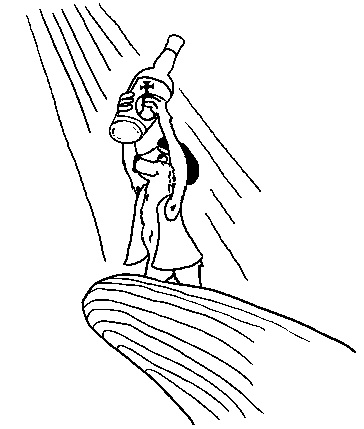
\includegraphics[width=0.7\textwidth]{images/chartreuse.jpg}
\end{center}

\breakpage